\section{Versuchsaufbau}
Der Versuch ist aus vier Grundbausteinen aufgebaut die in Abbildung \ref{fig:versuchsaufbau}
gezeigt sind. Dabei bilden ein Permanentmagnet, ein digitales Speicheroszilloskop sowie ein
PS2-Controller und ein Steuermodul die Hauptbestandteile.
\begin{figure}
    \center
    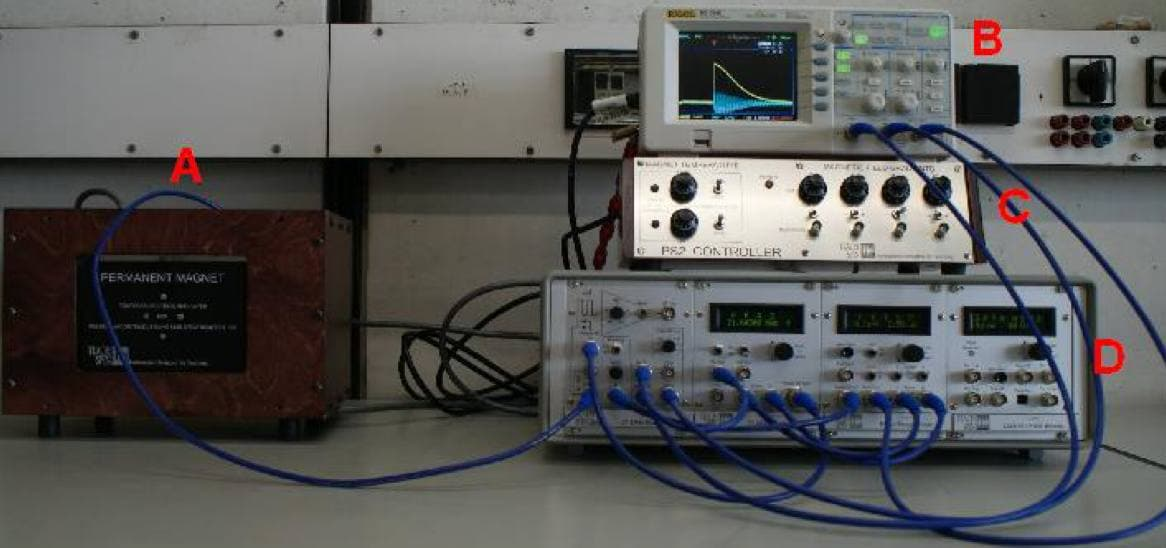
\includegraphics[width=0.8\textwidth]{bilder/versuchsaufbau.jpg}
    \caption{Dargestellt ist der Versuchsaufbau mit einem Permanentmagneten A, einem digitales Speicheroszilloskop B, einem
    PS2-Controller C und einem Steuermodul D\cite{anleitung}}
    \label{fig:versuchsaufbau}
\end{figure}
\subsection*{21 MHz Synthesizer}
Damit lässt sich die Frequenz-Veränderung des rf-Impulses variieren.
\subsection*{Impuls Programmierer}
Der Impuls kann darüber hinaus mit dem Programmierungs-Baustein weiter modifziert werden.
Dabei kann die Länge der jeweiligen Impulse sowie die Anzahl und Wiederholzeit der IMpulssequenz eingestellt werden.

\section{Durchführung}
\label{sec:Durchfuehrung}
